\documentclass[conference]{IEEEtran}
\IEEEoverridecommandlockouts
% The preceding line is only needed to identify funding in the first footnote. If that is unneeded, please comment it out.
\usepackage[a4paper, top=19mm, bottom=43mm, left=14.3mm, right=14.3mm]{geometry} 
\usepackage{cite}
\usepackage{float}
\usepackage{amsmath,amssymb,amsfonts}
\usepackage{algorithmic}
\usepackage{graphicx}
\usepackage{textcomp}
\usepackage{colortbl}
\usepackage{tabularray}
\UseTblrLibrary{booktabs}
\usepackage{xcolor}
\def\BibTeX{{\rm B\kern-.05em{\sc i\kern-.025em b}\kern-.08em
    T\kern-.1667em\lower.7ex\hbox{E}\kern-.125emX}}
\begin{document}

\title{Automatic Question Generation from Handwritten 
Lecture Notes Using TrOCR Text Recognition and T5 
Language Processing}
\author{\IEEEauthorblockN{Rommel John Ronduen\textsuperscript{1}, Jan Adrian Manzanero\textsuperscript{2}, Analyn Yumang\textsuperscript{3}}
\IEEEauthorblockA{\textit{School of Electrical, Electronics, and Computer Engineering} \\
\textit{Map\'ua University}\\
Manila, Philippines 1002\\
\textsuperscript{1}\texttt{rjhronduen@mymail.mapua.edu.ph}\\ 
\textsuperscript{2}\texttt{jacmanzanero@mymail.mapua.edu.ph}\\ 
\textsuperscript{3}\texttt{anyumang@mapua.edu.ph}}
}


\maketitle

\begin{abstract}
    \indent This research involves the creation and evaluation of a system that allows 
    for text extraction and automatic question generation (AQG) using a 
    Text-to-Text transformer (T5) and Transformer-based 
    Optical Character Recognition (TrOCR) pipeline. It addresses 
    the lack of OCR implementation with AQG alongside
    handwritten notes as the basis for questions generation. 
    With the use of a Raspberry Pi 5, web camera, 
    and a touchscreen display, factoid-type questions are created from image captures of 
    single-column handwritten notes that only contain 
    textual information. The 
    T5 large language model (LLM) used was 
    fine-tuned using the 
    Stanford Question Answering Dataset (SQuAD) for 
    facilitating question 
    generation. Evaluation was done using the word error rate (WER)
    for OCR, while 
    the Recall Oriented Understudy for Gisting Evaluation (ROUGE) 
    and Bilingual Language Evaluation Understudy (BLEU) metrics 
    were used for AQG. The system had a WER of 
    0.40, a ROUGE-1 score of 0.358, and a question validity rate of 
    68\% that led to questions with decent context 
    similarity versus student-made questions. It is recommended that better hardware is to be used, 
    consequently allowing for larger 
    versions of T5 and
    TrOCR. Moreover, much emphasis should be made with 
    the OCR proprocessing.
\end{abstract}

\begin{IEEEkeywords}
\indent Large Language Model, Optical Character Recognition,
Automatic Question Generation, Handwritten Lecture Notes, Raspberry Pi
\end{IEEEkeywords}

\section{Introduction}
\IEEEPARstart{H}{}andwritten lecture notes can be considered as the standard way 
for capturing and facilitating learning. These lecture notes are 
learning artifacts that may contain valuable information that can 
be the basis for other learning elements. One of these learning elements 
involve review questions. These questions are collected in the 
form of quizzes and question banks that allow for the enforcement of 
learning across various fields. Since the introduction of artificial 
intelligence (AI) to education, there have been several advancements 
that are attributed to improving the learning experience of students. 
Automatic question generation (AQG) is one of such advancements. 
It is achieved using large language models (LLMs) from various inputs 
that created questions for the assessment or learning enforcement of 
students.
\\
\indent Despite feasibility in AQG systems, 
these cannot process handwritten notes 
due to the lack of integrated optical character recognition (OCR) 
\cite{Arbaaeen2020}. AQG is derived from LLMs 
such as Text-to-Text Transformer (T5), Bidirectional Encoder Representations from Transformers 
(BERT), and Generative Pre-trained Transformer 3 (GPT-3), which have use cases from 
treebanks \cite{Mesina2020} and classification of certain texts \cite{Padilla2020} \cite{Mingua2021} \cite{Fernandez2023}.
Existing AQG frameworks are categorized by 
their information processing methods, yet none address 
handwritten sources \cite{Arbaaeen2020}. While \cite{Ou2022} demonstrated AQG 
on videos using BERT for named entity recognition (NER) on 
transcribed audio, textual or handwritten contexts remain 
unexplored. Other approaches include manual text input 
with part-of-speech (POS) tagging \cite{Moron2021}, rule-based methods 
for programming code \cite{Gaur2023}, and the T5 model 
fine-tuned on SQuAD for text-based AQG \cite{Tsai2021}. OCR, defined as 
image-to-text conversion via convolutional neural networks (CNNs) \cite{Ligsay2022}, has been applied to handwritten Baybayin \cite{Ligsay2022}, medicinal mushroom classification \cite{Sutayco2024}, and expiry date extraction \cite{Manlises2024}. Through \cite{Calimag2023}, a use case combined CNNs with 
recurrent neural networks (RNNs) for real-time inference, evaluated via confusion matrices \cite{Ishikawa2020} \cite{Villaverde2023}. However, Transformer-based OCR (TrOCR) 
\cite{Li2021}, pre-trained on the IAM Handwriting Database, offers superior paragraph-level text recognition over character-
focused CNNs \cite{Mortadi2023}. TrOCR’s robustness positions it as a critical enabler for AQG from handwritten lecture notes, addressing the identified gap in media diversity \cite{Arbaaeen2020}. 
\\
\indent In bridging the gap for processing handwritten lecture notes for AQG, this research has the 
general objective of performing AQG from handwritten lecture
notes using TrOCR text recognition and T5 language processing.
Specifically, this research aims to extract text from
handwritten lecture notes using TrOCR and refine such text 
using the Gemini 1.5 Flash LLM; utilize 
a fine-tuned base version of T5 on SQuAD for AQG on 
indexed keywords from spaCy and Rapid Automatic Keyword 
Extraction (RAKE) on the refined text; utilize a Raspberry 
Pi 5 within a constructed enclosure with illumination 
for facilitating the system processes and experimental setup;
and lastly, to evaluate the system using the word error 
rate (WER) for the OCR, and the Recall-Oriented Understudy for 
Gisting Evaluation (ROUGE) and the Bilingual Language Understanding 
Evaluation (BLEU) for the comparison of AQG to the 
student-generated questions.
\\
\indent This system only considers handwritten lecture notes 
that are single-column, diagram and equation free, and written 
in English on plain sheet letter-size paper. It is important to note that 
this system utilizes the base versions of the T5 and TrOCR models where the 
former uses SQuAD for the fine-tuning and Gemini 1.5 Flash for the 
text correction and context completion of OCR-extracted text as well as 
the spaCy-Rake keyword extraction for AQG basis. The system 
requires a single word to be detected to work, where it can 
produce a minimum of a single question up to five. Also, the system operation is confined 
within the processing capability of the 8-gigabyte model of the Raspberry Pi 5.
A different model for OCR or AQG may lead to differing results as well as 
for the text-enhancing model. Lastly, the usage of alternative hardware 
may lead to different results.
\section{Materials and Methods}
\subsection{Hardware development} 
\subsubsection{Block Diagram}
\hfill \\
\vspace{-0.4cm}
\begin{figure}[H]
\centerline{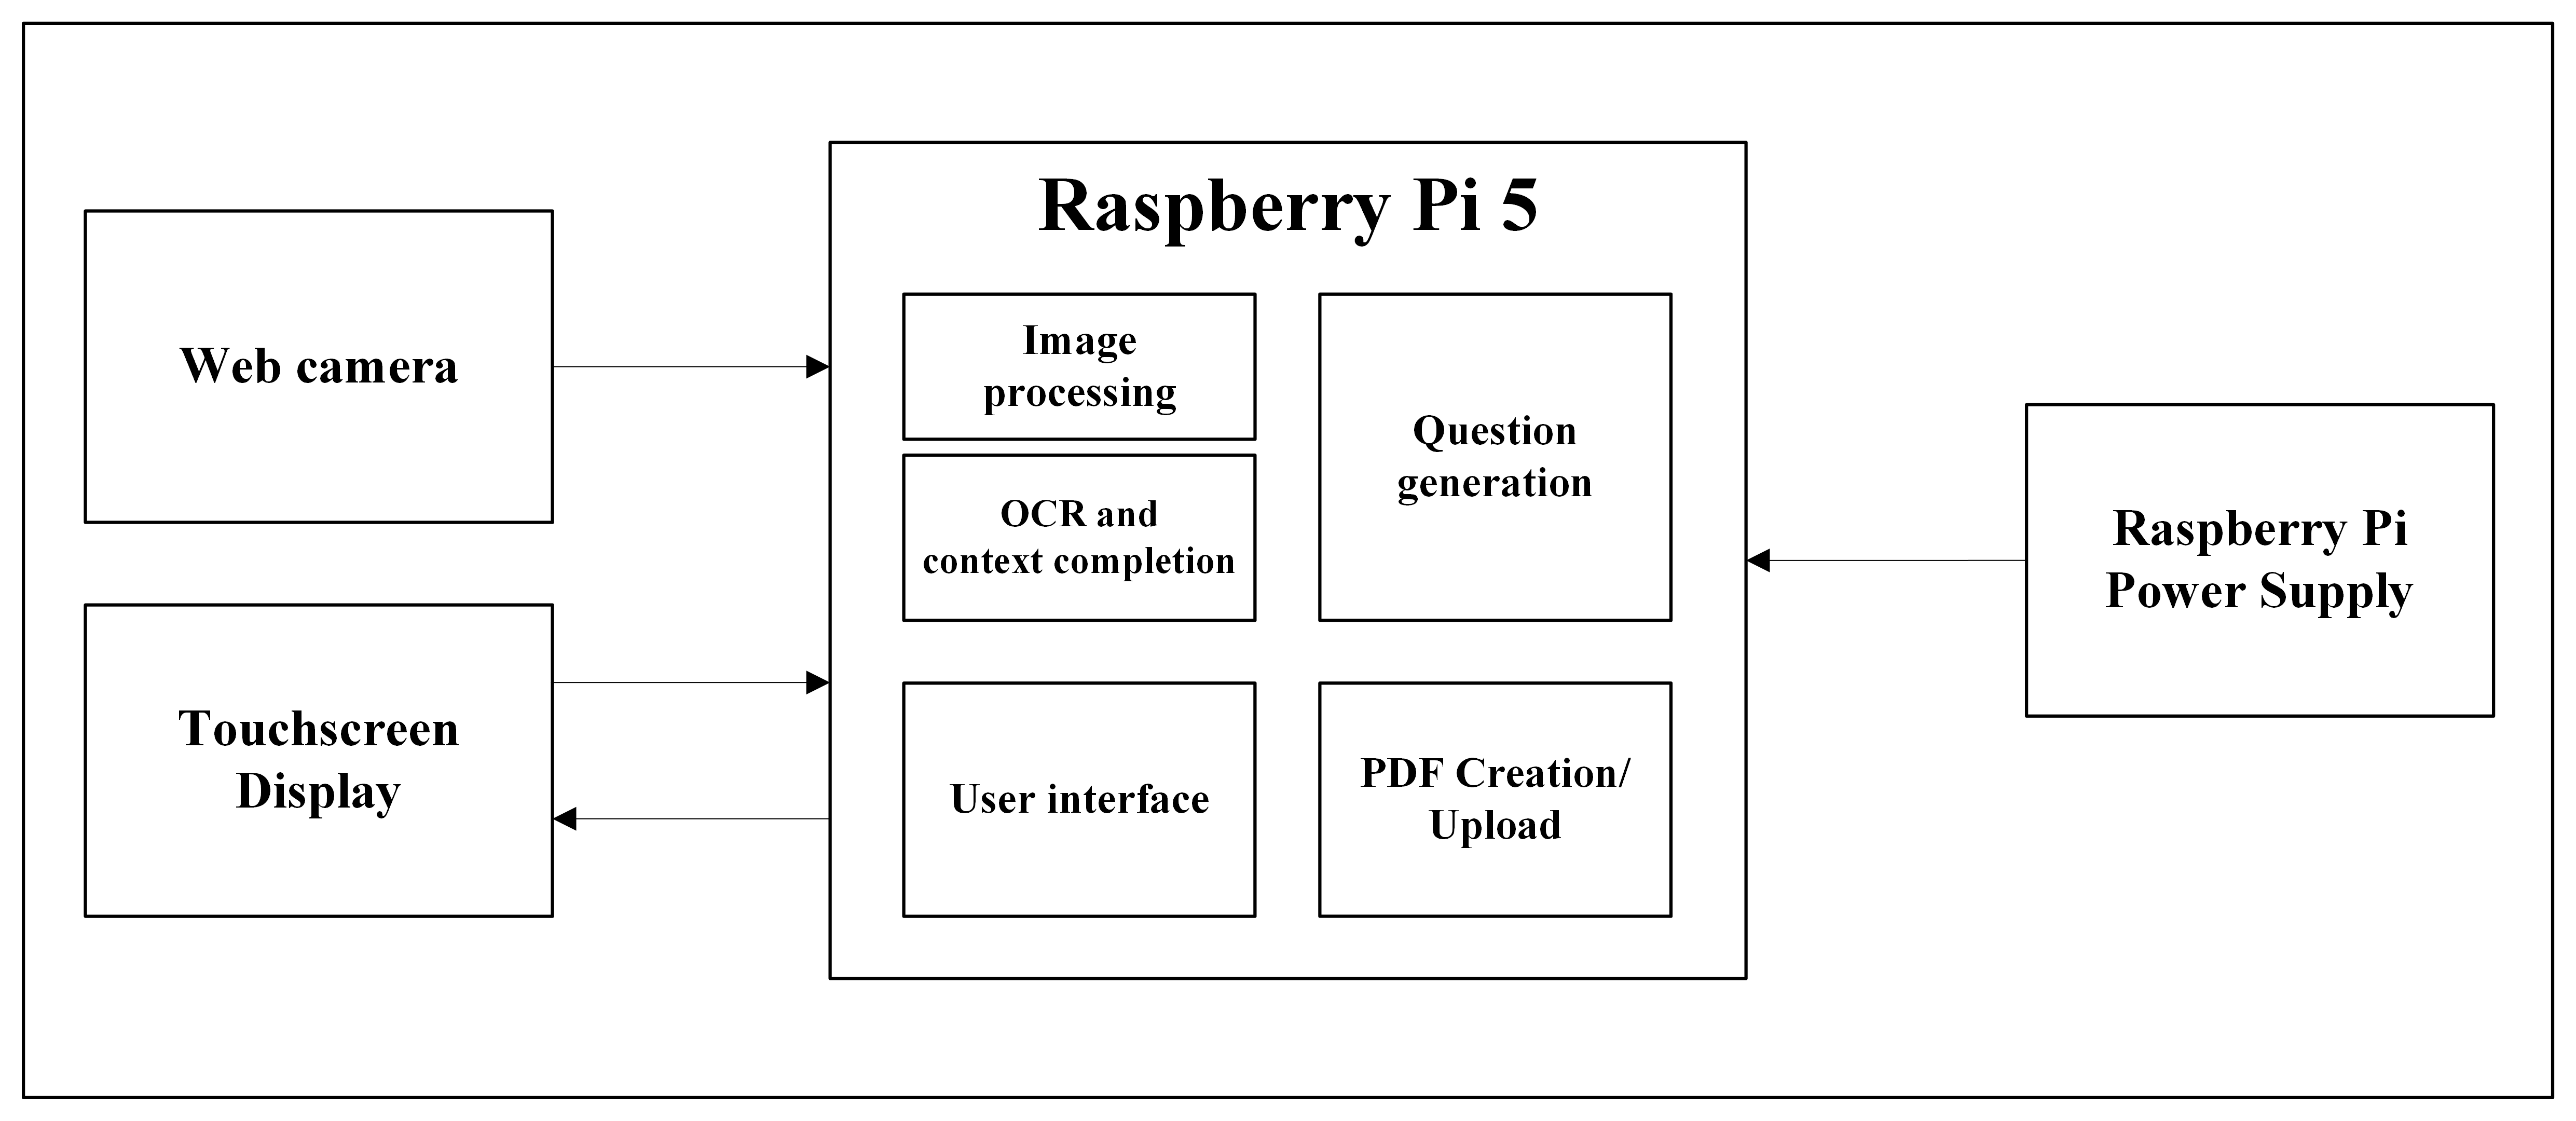
\includegraphics[width=0.5\textwidth]{blockdiag.png}}
\vspace{-0.4cm}
\caption{System block diagram.} 
\label{blockdiag}
\end{figure}
\indent Fig. \ref{blockdiag} is an illustration for the interconnections 
of the system. The Raspberry Pi 5 facilitates the system algorithm 
through the use of the web camera for the capture of handwritten notes and 
the touchscreen display for the user inputs in dictating the system 
operation. The power supply for the Raspberry Pi 5 allows for the delivery 
of power to the accessory components and main hardware of the system.
A Logitech C922 web camera was used that allowed for autofocus 
and a $1920\times 1080$ pixel capture resolution. Moreover a 
Waveshare $800\times480$ touchscreen liquid crystal display (LCD) 
allowed for the display while also providing tactile input.\\
\indent The services on the system were deployed using Docker as 
individual representation state transfer (REST) application programming 
interfaces (APIs). The front end was made using Angular where it acts 
as the collector of the images of handwritten notes through video feeds 
and interactive buttons. On the other hand, the back end used Flask 
that allows for API handling while also supporting the functions needed 
in facilitating the OCR and AQG processes. Lastly, a portable document 
format (PDF) file was to be made from the array of question strings that 
would be uploaded to Google Drive where a consequent download link 
will be displayed as a quick response (QR) code to the user in the 
front end.
\subsubsection{Experimental Setup}
\hfill \\
\begin{figure}[H]
\centerline{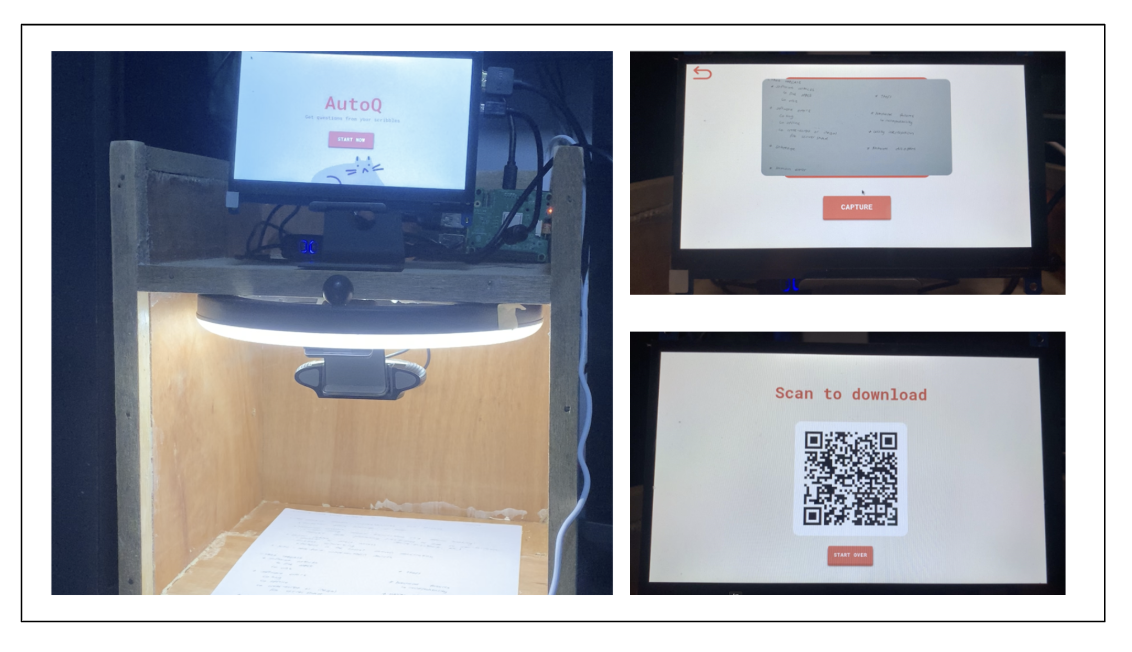
\includegraphics[width=3.6in]{experimental.png}}
\vspace{-0.4cm}
\caption{Constructed prototype and experimental setup.} 
\label{experimental_setup}
\end{figure}
\vspace{-0.3cm}
\indent The constructed prototype is shown in Fig. \ref{experimental_setup}.
Experimental setup is done where the system demands handwritten notes 
in the interior of the prototype. An internet connection is required for
the experimental setup. The user is then guided by the front-end 
to capture the handwritten notes. Two halves are captured for the
notes where the first half is the top half and the second half is the
bottom half. The user is then prompted to confirm the captured notes
for the system to proceed with the OCR operation. The system then
proceeds with the OCR operation and the AQG operation. The user is then
prompted to confirm the generated questions for the system to proceed
with the PDF generation. The user is then prompted to download the PDF
file for the generated questions.
\hfill
\subsection{Software development}
\subsubsection{Algorithm Pipeline}
\hfill
\begin{figure}[H]
\centerline{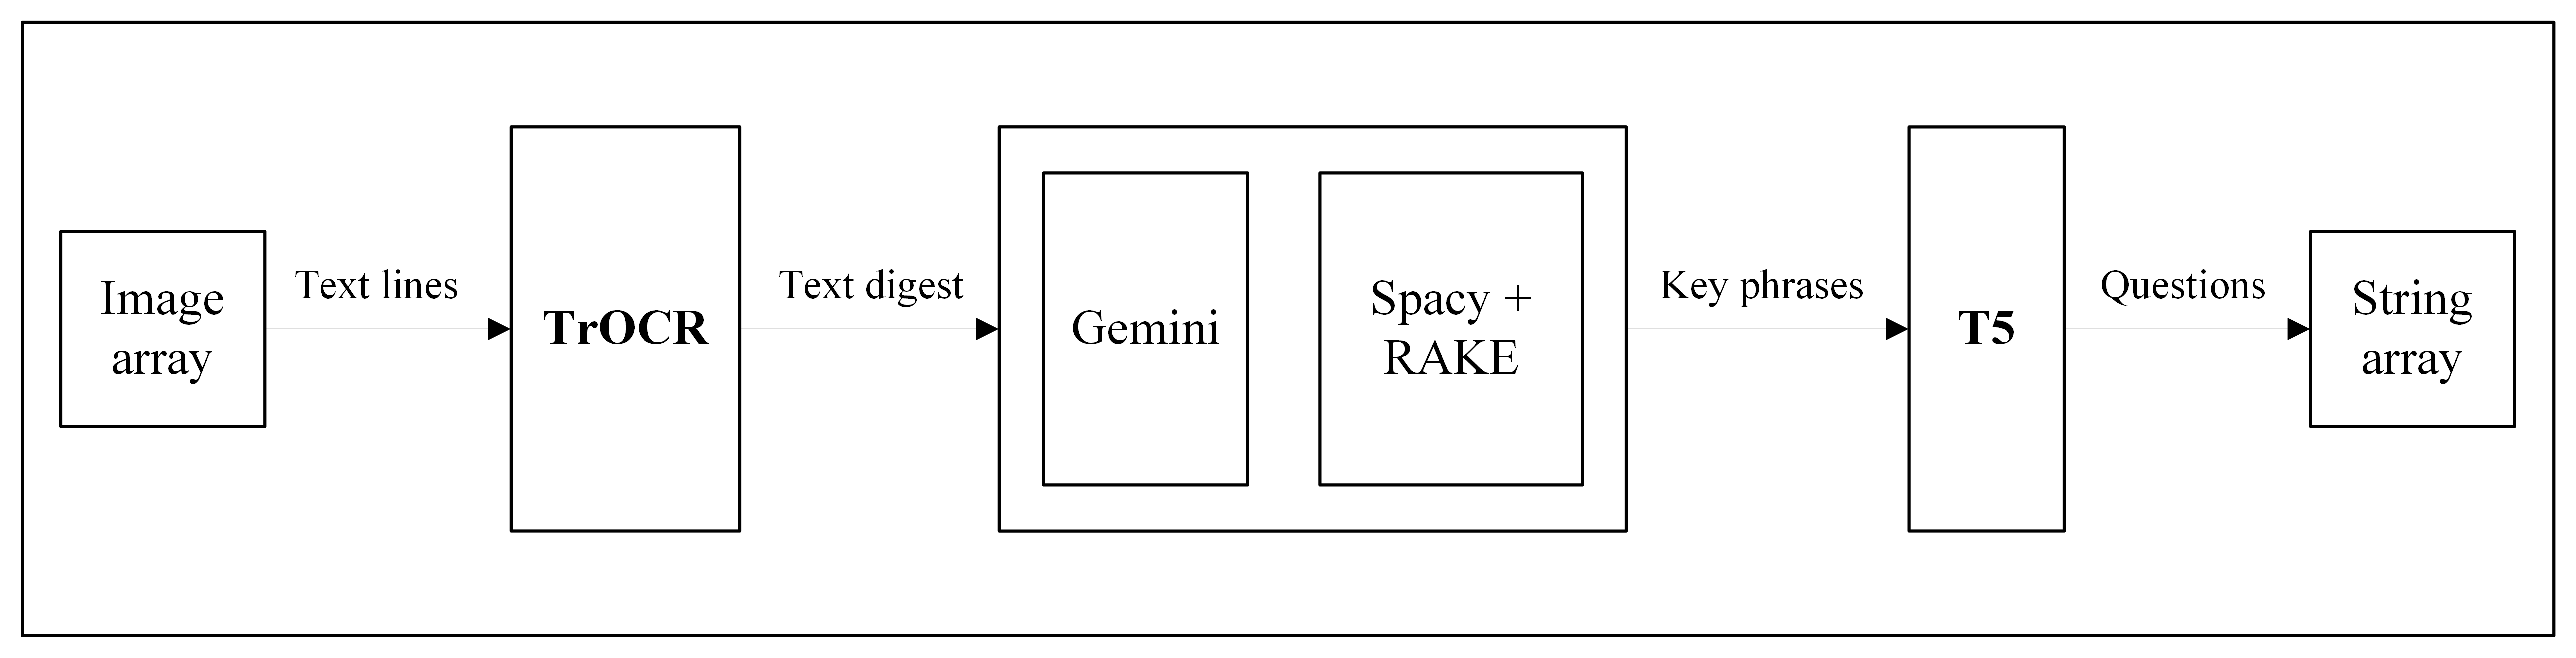
\includegraphics[width=3.5in]{pipeline.png}}
\vspace{-0.4cm}
\caption{Algorithm pipeline.} 
\label{pipeline}
\end{figure}
\indent Shown in Fig. \ref{pipeline} is the illustration 
of the step-by-step flow of information on the system 
algorithm. An image array in the memory of the system consists 
of the image captures of the handwritten lecture notes in the 
form of OpenCV image objects. These images undergo 
a series of fast means denoising, thresholding, and 
dilation to detect text lines. These text lines are stored in 
another array where TrOCR performs batch inferences to attempt 
extraction from the sources. spaCy and RAKE collected 
relevant keywords and phrases as a basis for the question generation 
which was sent to the T5 model for generation of questions. 
These questions are then stored in an array for portable document 
file (PDF).

\hfill
\begin{figure}[H]
\centerline{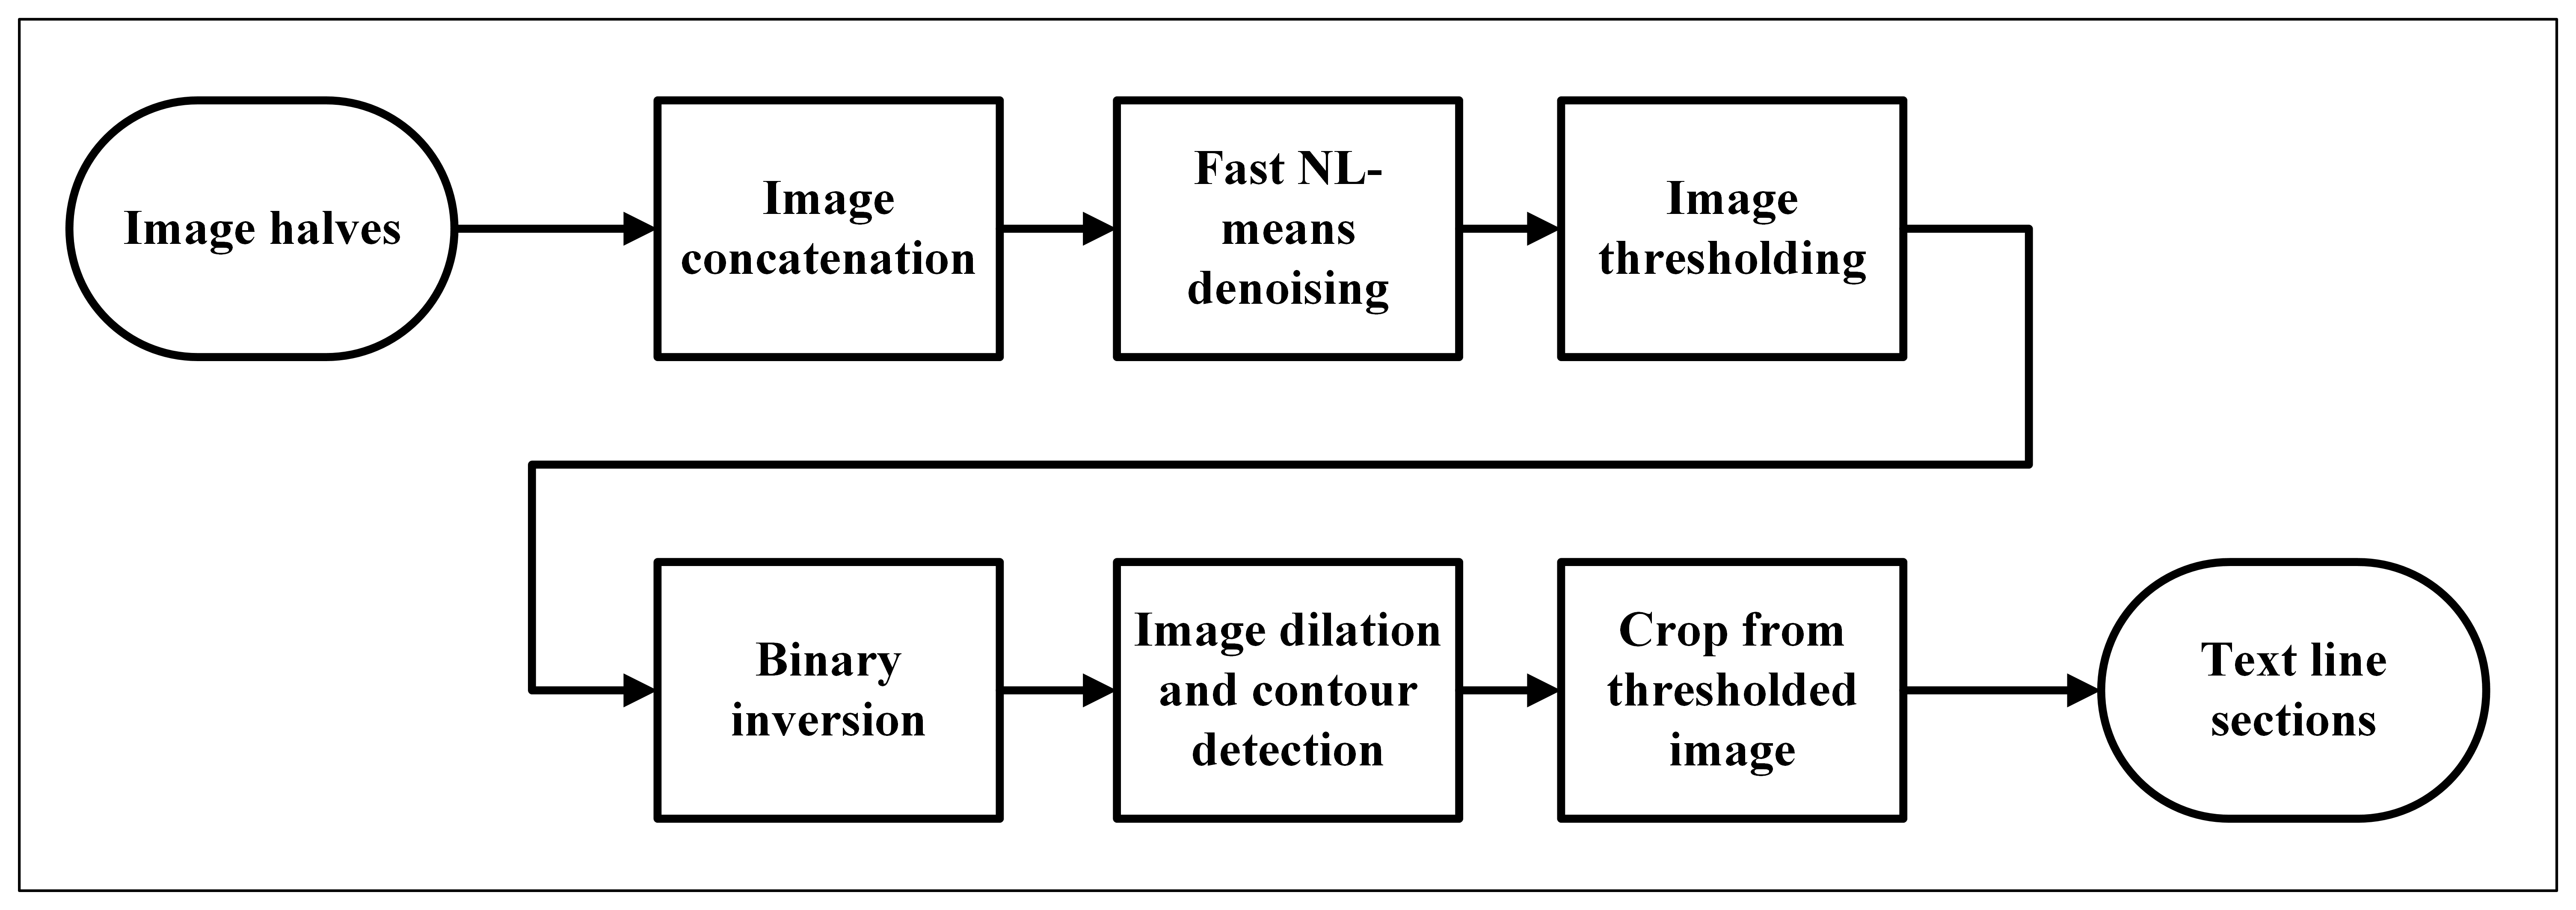
\includegraphics[width=3.5in]{ocr_process.png}}
\vspace{-0.4cm}
\caption{Text line detection and extraction process.} 
\label{ocr_process}
\end{figure}

\indent Revealed in Fig. \ref{ocr_process} is the step-by-step 
procedure for the process of retrieving text lines from 
a given document. It starts with the receiving of two half 
scans of a given document. Image concatenation involves 
the combination of the two to recreate the full document. 
Fast non-local (NL) means denoising and image thresholding 
converts the document scan to a more readable document while 
exposing the shape of the handwritten text. Image binarization 
and horizontal dilation allows for the reveal of text 
lines across the document. Finally, the detected text lines from the contours are cropped 
from the original image.
\hfill
\begin{figure}[H]
\centerline{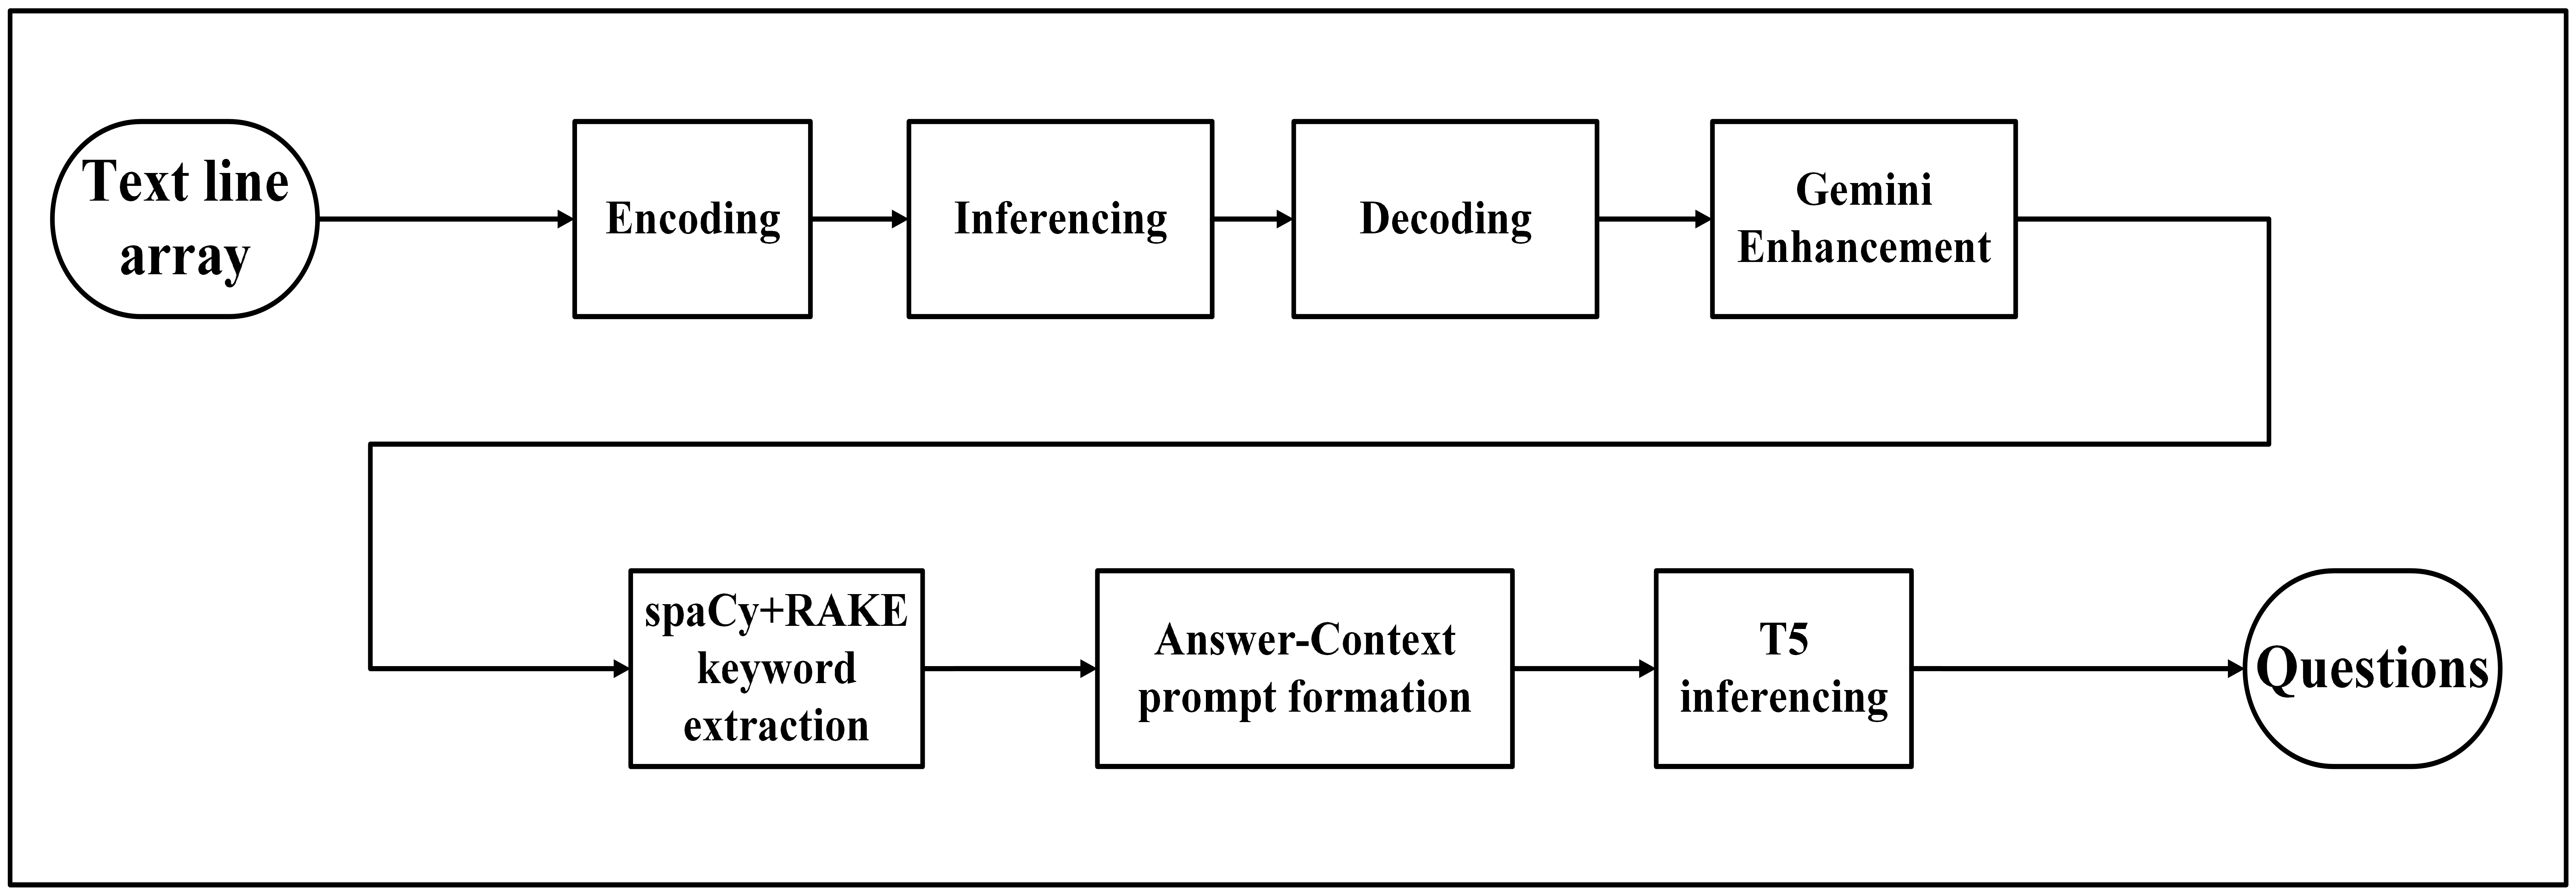
\includegraphics[width=3.5in]{trocr_process.png}}
\vspace{-0.4cm}
\caption{TrOCR and T5 processing.} 
\label{trocr_process}
\end{figure}
\indent In Fig. \ref{trocr_process}, it presents the detailed operation 
of TrOCR in the system. Coming from the extracted text line images 
from the process in Fig. \ref{ocr_process}, batch encoding, inferencing, and 
decoding was done on the array of text lines using the encoder-decoder 
framework provided by TrOCR. After the extraction procedure, it is 
prompted to Gemini where error correction is attempted from the 
OCR extraction. Coming from enhanced text in Fig. \ref{trocr_process}, 
the spaCy library and the RAKE algorithm was used to find the 
relevant keywords and phrases from the text as basis for the questions. 
Consequently, answer-context pairs are used as prompts that are inputted 
to the T5 model that generates the questions in an array. 
\vspace{0.3cm}
\subsubsection{Model Training}
\hfill \\ 
\indent The T5 base model was fine-tuned to the SQuADv1.1 
dataset for the AQG operation with a learning rate of 
$3 \times 10^{-5}$ for eight epochs using the Sequence2Sequence 
trainer. The SQuADv1.1 dataset was loaded using the
datasets library where the chosen input features 
were the context and the question. The output feature 
was the answer for the given pair of inputs.

\subsection{Data Collection}
\vspace{-0.2cm}
\begin{figure}[H]
\centerline{\includegraphics[width=3in]{datacollection.png}}
\vspace{-0.3cm}
\caption{Sample from the test set. Combined image vs. preprocessed image} 
\label{datacollection}
\end{figure}
\indent Shown in Fig. \ref{datacollection} is a sample 
from the test set containing 70 handwritten notes collected from undergraduate
classes on computer networks and cybersecurity. These notes were
written in English, single-column, and diagram-free. A total of
1800 individual text lines were extracted from the notes for the
evaluation of the OCR operation through manual transcription
and were saved in a comma-separated value (CSV) format for 
analysis. As part of the system operation on the 70 handwritten notes, 
350 questions (five questions per page) were produced for 
evaluation. \\
\indent Moreover, 135 questions were collected from the students that wrote the 
notes. The top five most common keywords from the overall extracted text 
(MAC, ethernet, address, data, and frame) were utilized as the basis 
for the questions alongside a summary written from the extracted notes 
that contained such keywords. 
\subsection{Testing and Evaluation}
\vspace{-0.2cm}
\begin{table}[H]
\caption{Testing and Evaluation Table for OCR.}
    \centering
    \begin{tblr}{
        colspec={@{}X[1] X[1] X[1] X[1]@{}}, % Makes columns flexible
        column{1} = {c}, % Align first column to center
        hlines,          % Adds horizontal lines
    }
    & \textbf{Student} & \textbf{Model} & \textbf{WER} \\
    1 &  &  &  \\
    ... & ... & ... & ... \\
    70 &  &  &  \\
    &  &   &  Average\\  % Replace X, Y, Z with actual values
    \end{tblr}
    \label{ocrtable}
\end{table}
\indent Shown in Table \ref{ocrtable} is the evaluation of the OCR operation
using the word error rate (WER) for the 70 handwritten notes. 
Testing is done through the collection of the transcribed 
text versus the inference of the model. The WER is
calculated using the formula:
\begin{equation}
    WER = \frac{S + D + I}{N}
\end{equation}
where $S$ is the number of substitutions, $D$ is the number of deletions, $I$ is the number of insertions, and $N$ is the number of words in the reference text.
\begin{table}[H]
    \caption{Testing and Evaluation Table for AQG.}
        \centering
        \begin{tblr}{
            colspec={@{}X[1] X[1] X[1] X[1] X[1]@{}}, % Makes columns flexible
            column{1} = {c}, % Align first column to center
            hlines,          % Adds horizontal lines
        }
        & \textbf{Student} & \textbf{Model} & \textbf{ROUGE} & \textbf{BLEU}\\
        1 &  &  &  & & \\
        ... & ... & ... & ... & ... \\
        135 &     &     &     &     \\ 
          &  &  &   Average & Average & \\  % Replace X, Y, Z with actual values
        \end{tblr}
        \label{aqgtable}
        \end{table}
\indent Shown in Table \ref{aqgtable} is the evaluation of the AQG operation
using the Recall-Oriented Understudy for Gisting Evaluation (ROUGE) and the
Bilingual Evaluation Understudy (BLEU). Data collection allowed for 
the accumulation of 135 questions from students. Using the top five 
keywords from the handwritten lecture notes, 
it is compared with the model-generated results using the basis keyword 
and context. ROUGE and BLEU are computed as 
follows:
\begin{equation}
    ROUGE = \frac{1}{N} \sum_{i=1}^{N} \frac{2 \times (P \times R)}{(P + R)}
\end{equation}
\begin{equation}
    BLEU = \frac{1}{N} \sum_{i=1}^{N} \frac{1}{r} \sum_{i=1}^{r} \min \left( \sum_{i=1}^{r} \text{count}_{\text{clip}}(ngram) \right)
\end{equation}
where $P$ is the precision, $R$ is the recall, $N$ is the number of notes, $r$ is the number of reference questions, and $\text{count}_{\text{clip}}$ is the count of the clipped n-grams.
\section{Results and Discussion}
\begin{figure}[H]
    \centerline{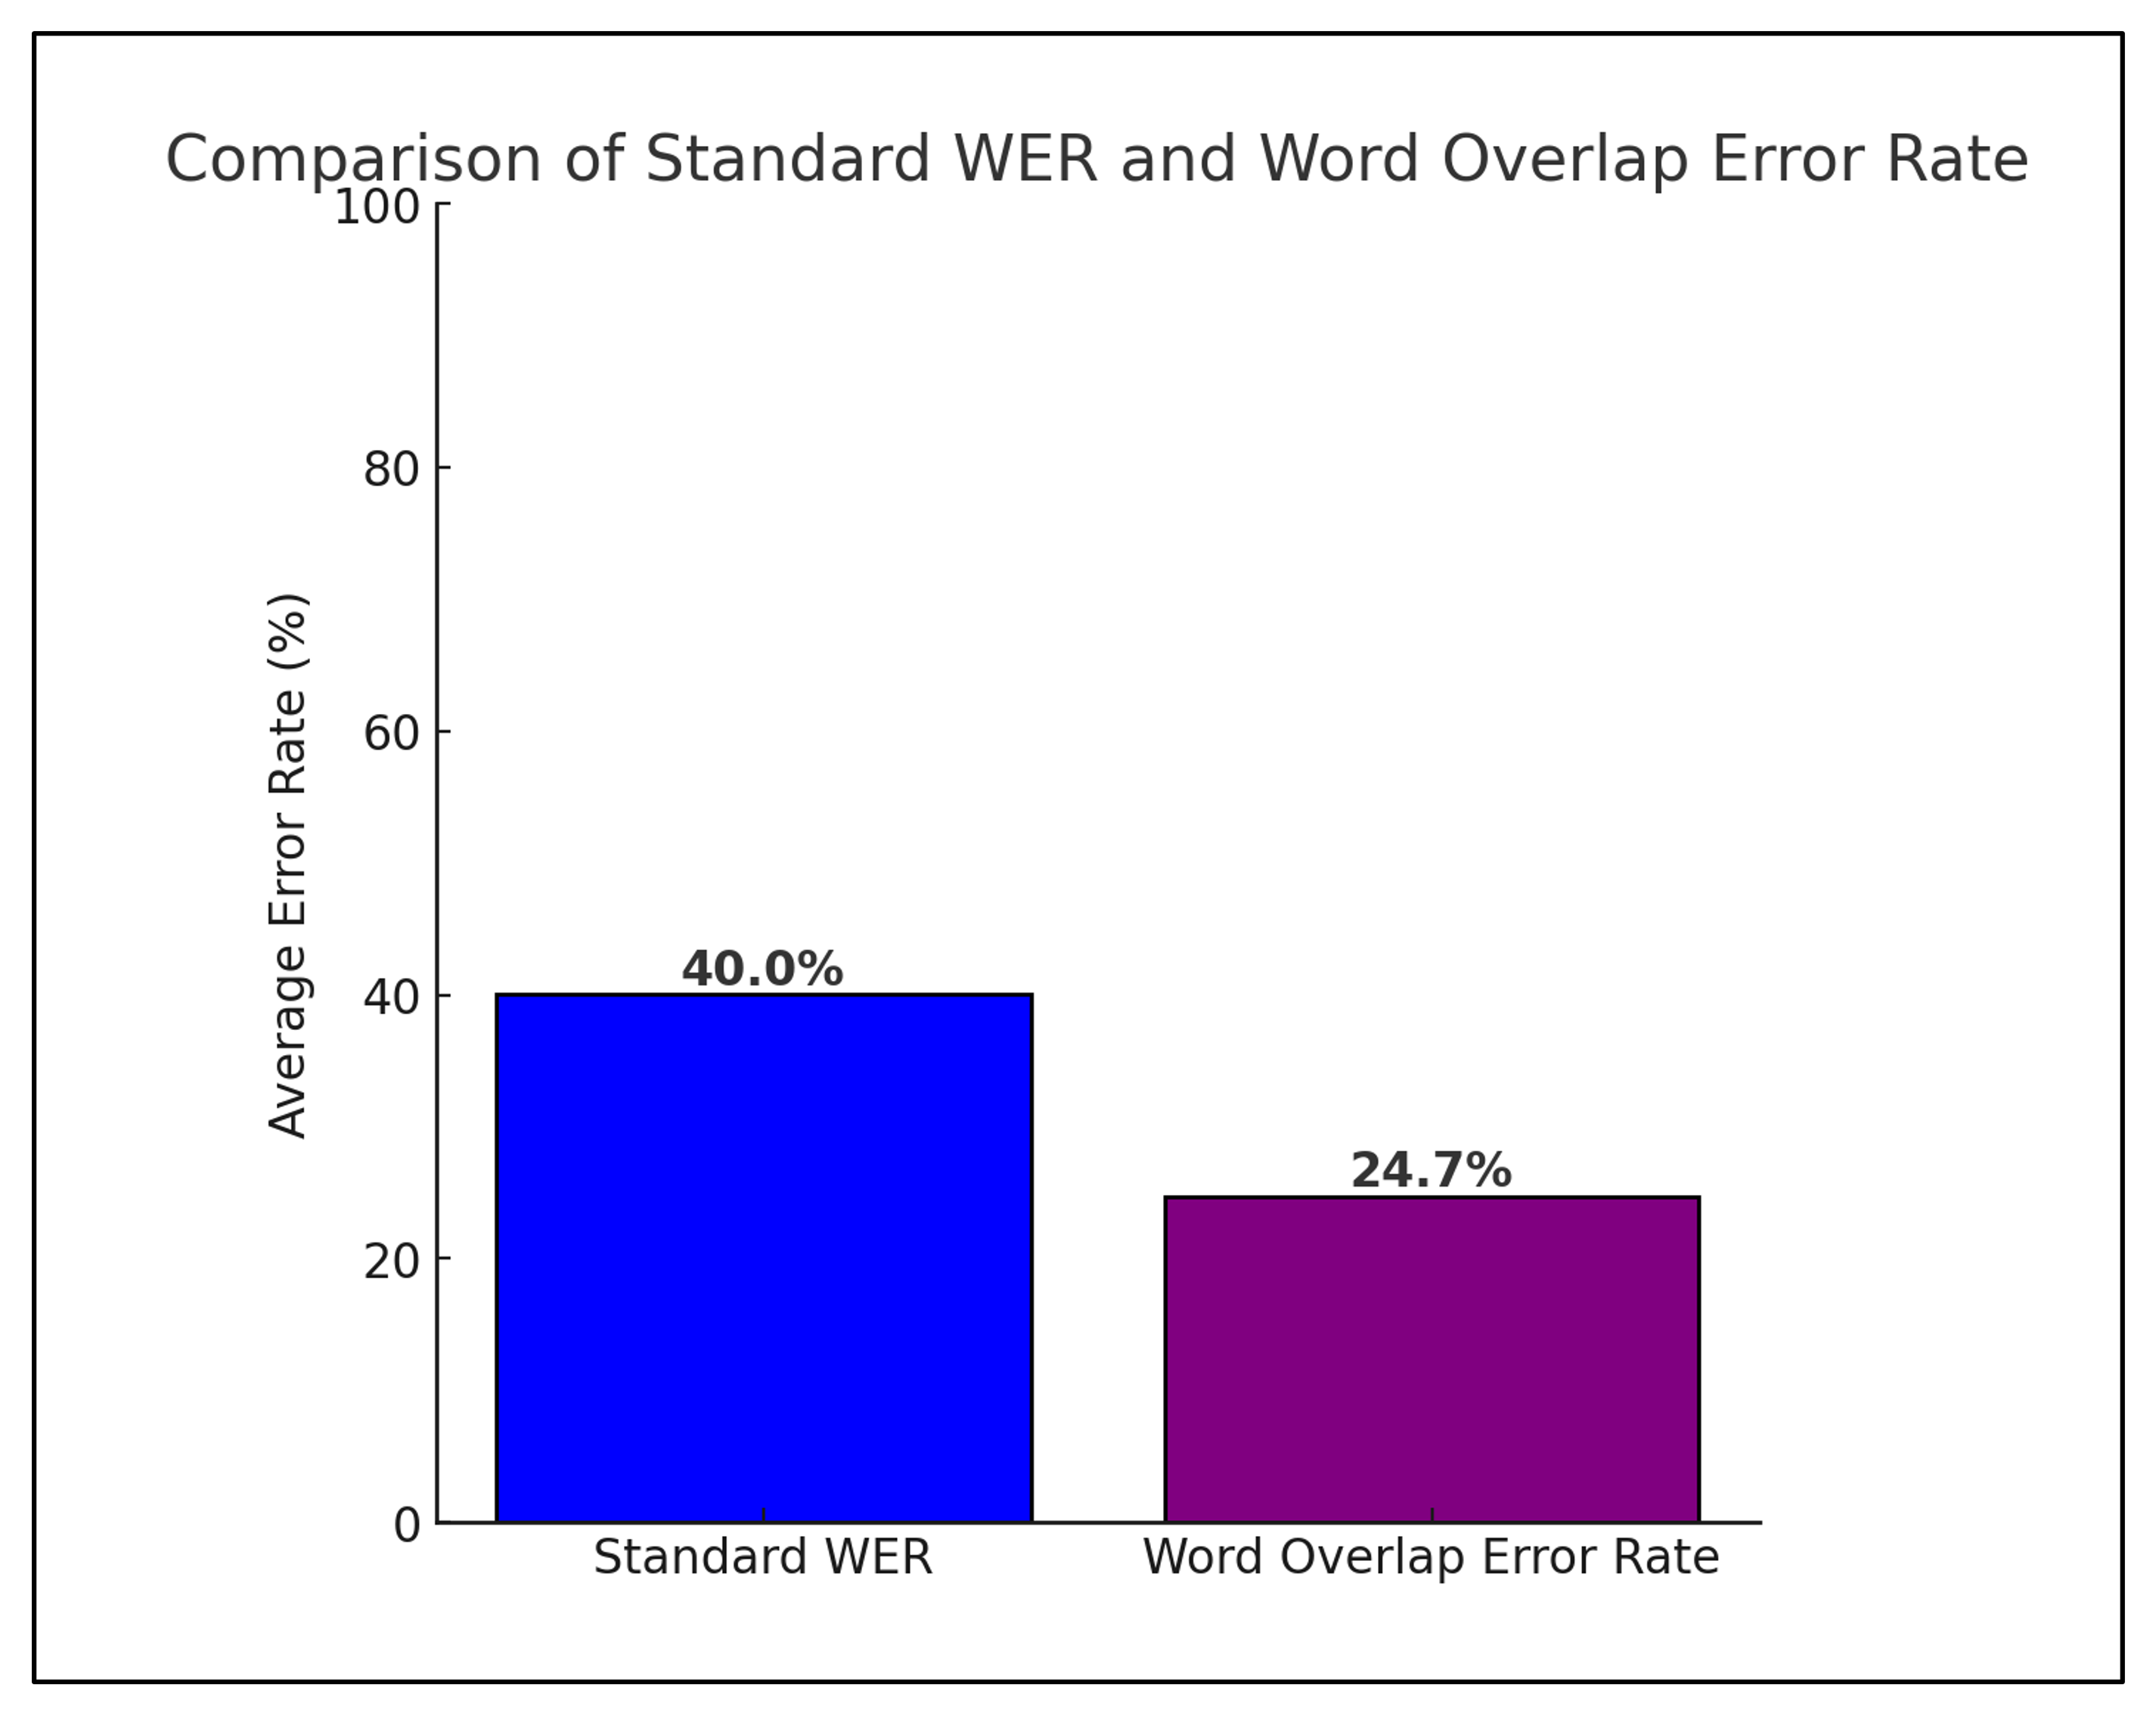
\includegraphics[width=2.5in]{wer.png}}
    \vspace{-0.4cm}
    \caption{Computed WER and WOER} 
    \label{wer}
    \end{figure}
\indent In Fig. \ref{wer}, it was shown that a WER of 0.40 or 40\% 
was realized from the implementation of the TrOCR model with a 
word overlap error rate (WOER) of 0.247 or 24.7\% that 
measures the completeness of the inference versus the reference.
The relatively moderate magnitude of the WER was realized due to the 
natural misalignment of the text lines from the handwritten notes. 
Moreover, the lack of use-case specific fine-tuning to TrOCR 
may have contributed to the WER magnitude. Nevertheless, the
the 60\% accuracy allowed enough room for Gemini 1.5 Flash to correct 
and bridge the gaps in the text digest to form valid questions.
\begin{figure}[H]
    \centerline{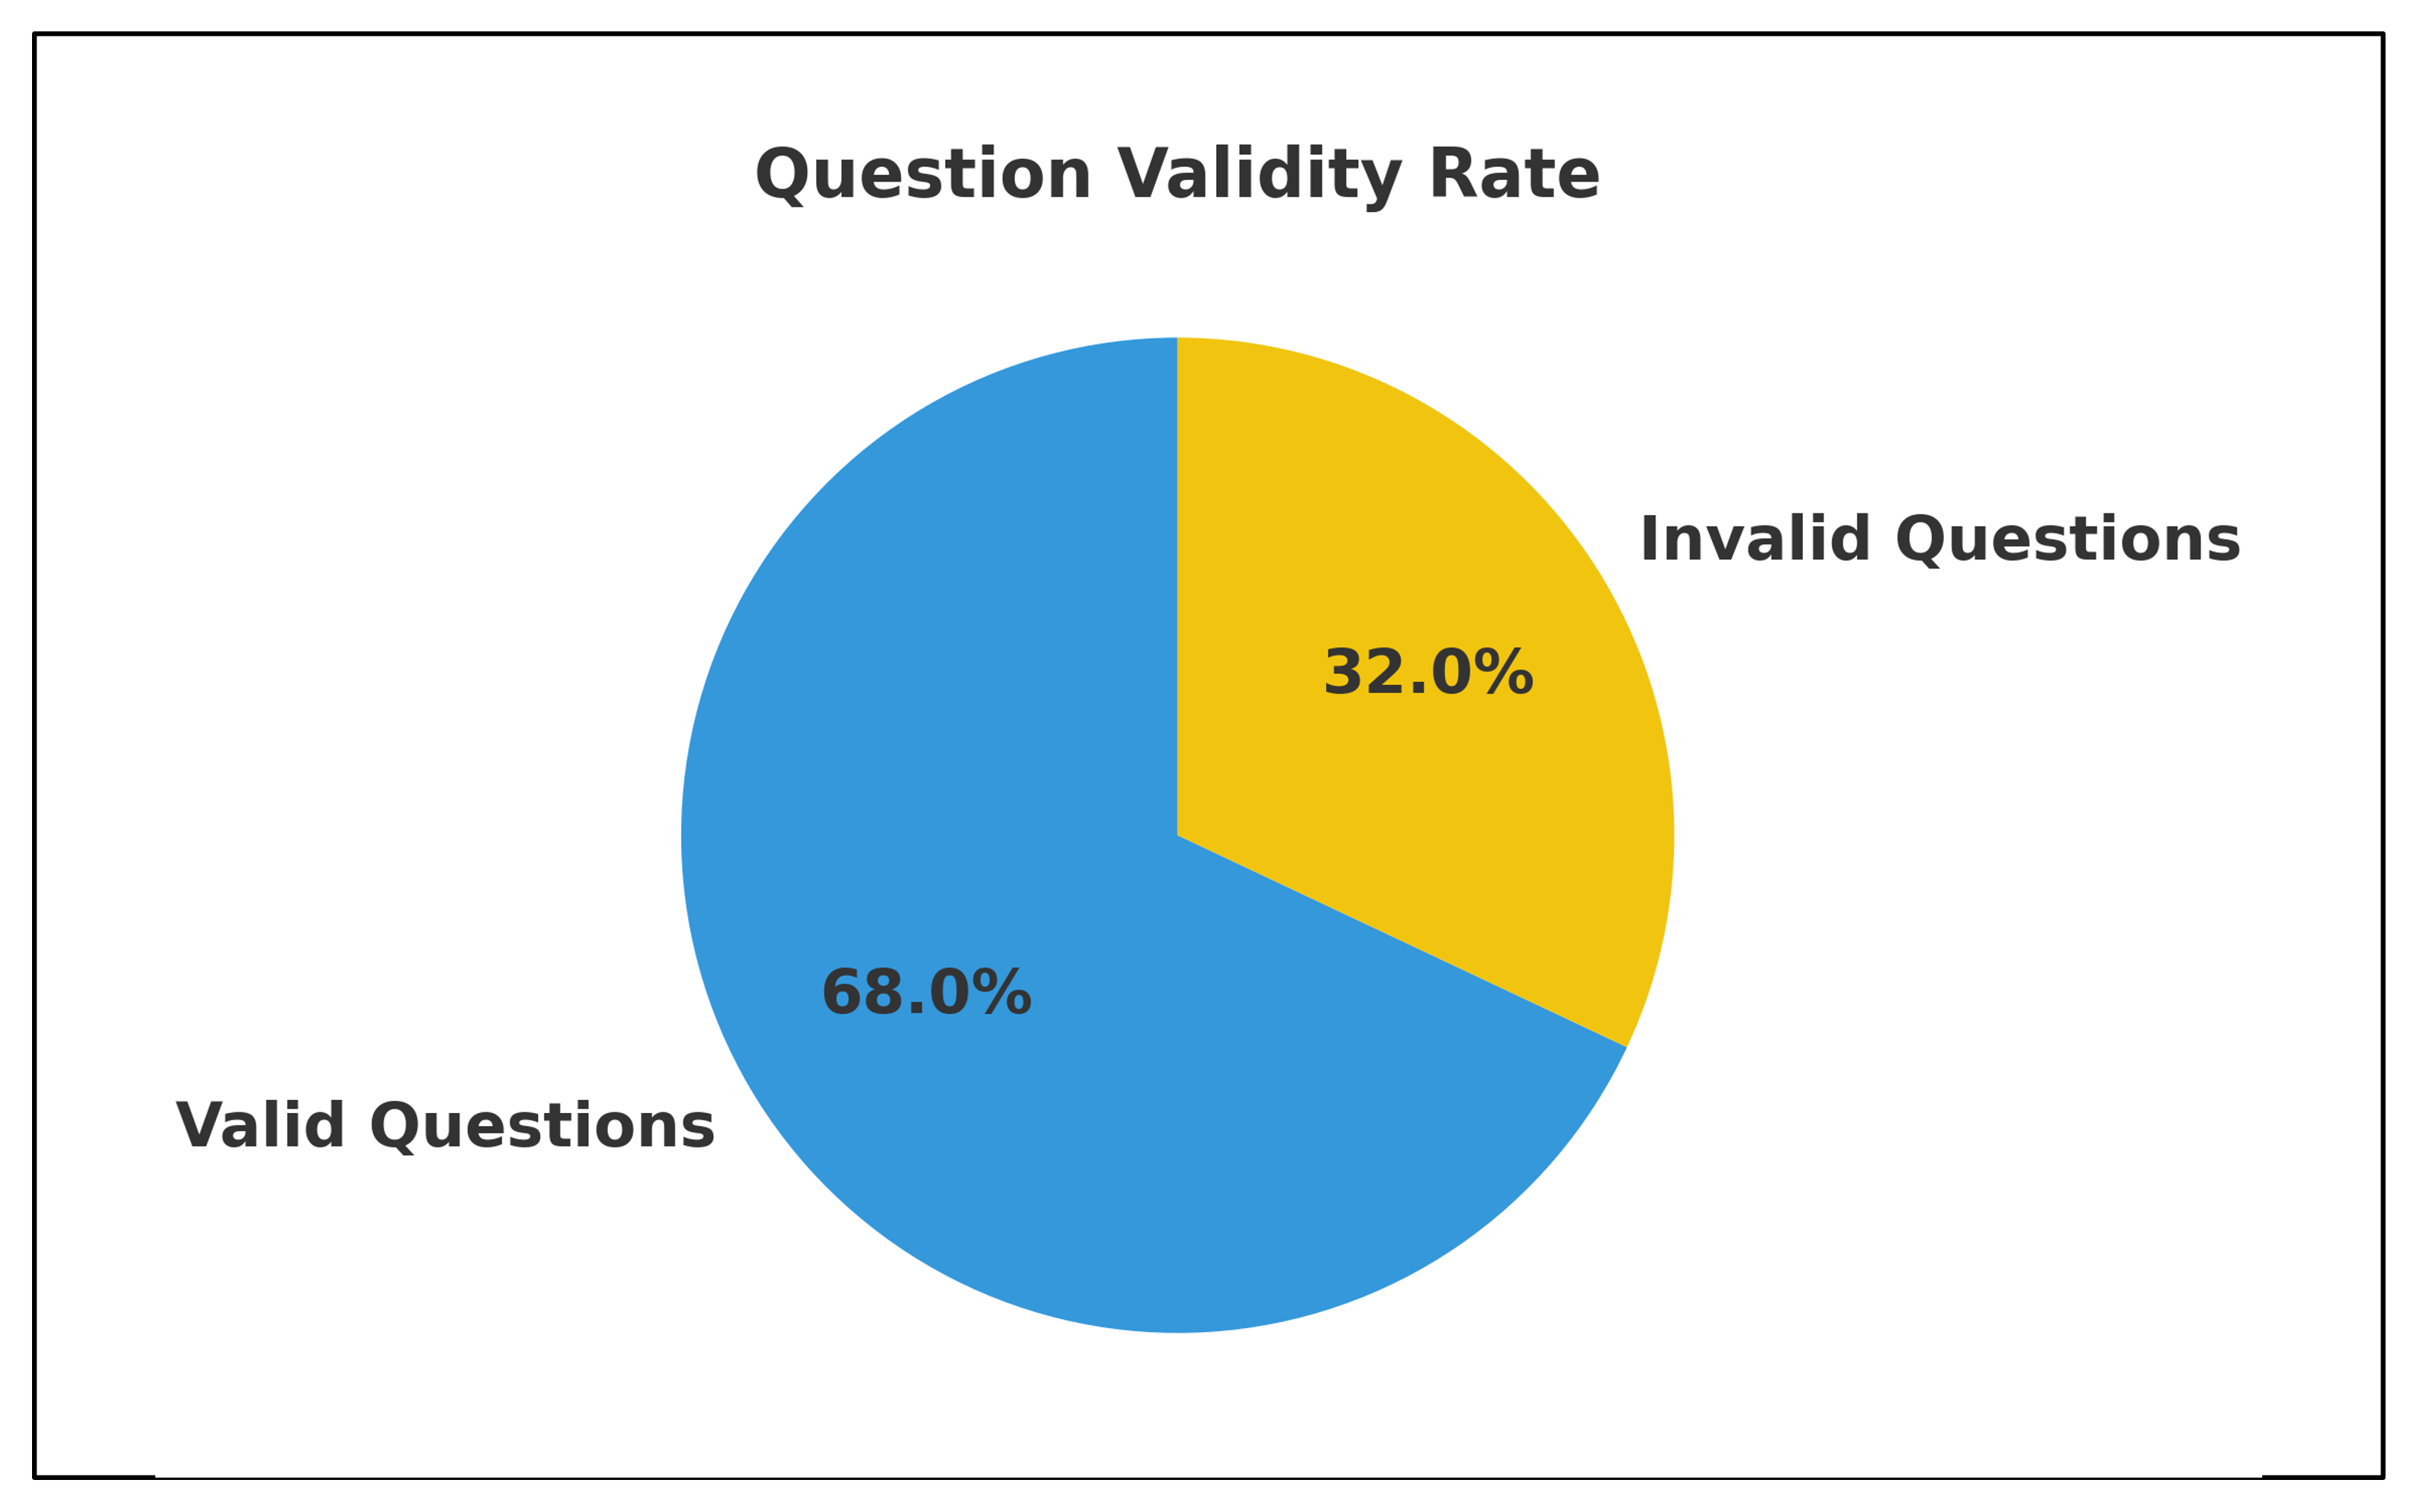
\includegraphics[width=3in]{validity.png}}
    \vspace{-0.3cm}
    \caption{Question Validity Rate Pie Chart} 
    \label{validity}
    \end{figure}
\indent In Fig. \ref{validity}, it revealed that the generated questions 
by the system are valid 68\% of the time where out of 350 questions, 
238 were valid in terms of coherency, grammar, and it's correlation 
to the subject matter. The remaining invalidity of 32\% was attributed to 
possibly two aspects. First, the T5 model may need additional 
parameters such that of the large or extra large (XL) model 
to generate better questions. The second is that some keywords may have not been 
corrected by the Gemini 1.5 Flash model which may have led to the
propagation of errors in the generated questions.
\begin{figure}[H]
    \centerline{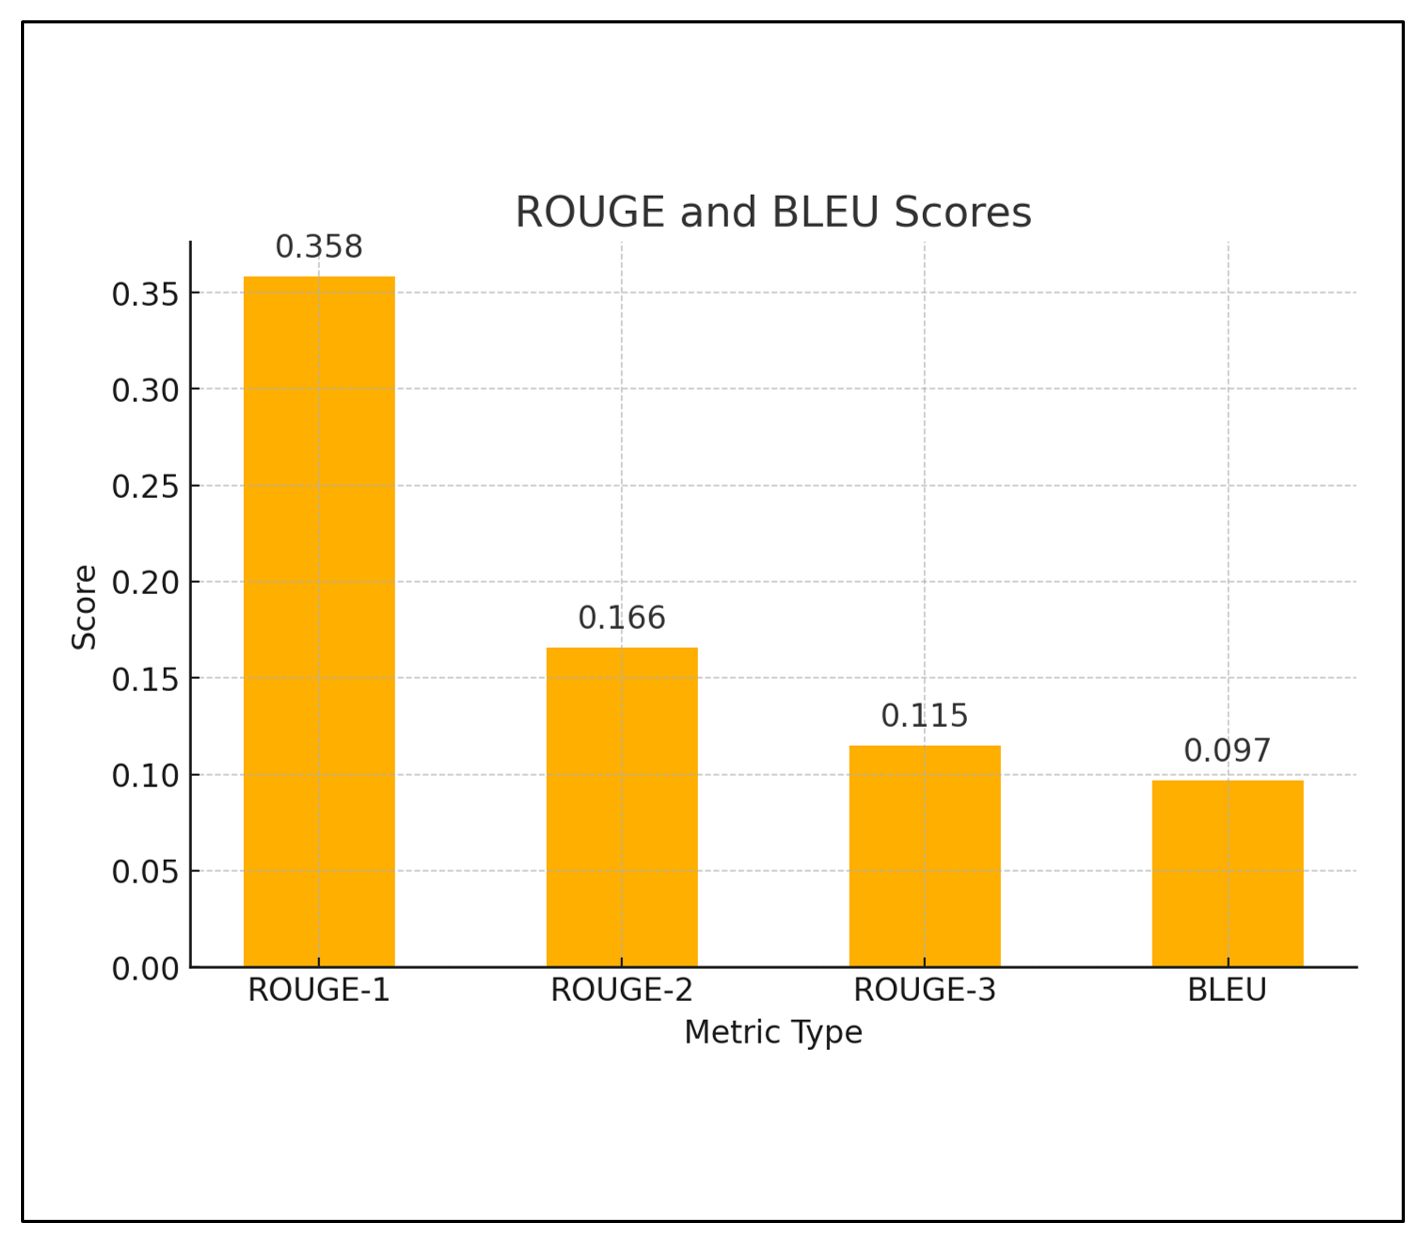
\includegraphics[width=2.5in]{eval.png}}
    \vspace{-0.3cm}
    \caption{ROUGE scores and BLEU evaluation} 
    \label{eval}
\end{figure}
\vspace{-0.3cm}
Shown in Fig. \ref{eval} is the evaluation of the AQG operation by means
of the ROUGE scores and the BLEU scores. 
It is important to settle first that the questions made by the 
students tend to be verbatim copies of the basis context. 
A ROUGE-1 score of 0.358 meant that the system decently captures 
the relevant keywords in the same way as students do. 
Moreover, the ROUGE scores 0.166
and 0.115 meant model-based questions differ from the 
students by syntax
because much students verbatimly copy 
the structure of the context compared to the dynamic outputs 
of the system. Lastly, the BLEU score of 0.097 meant that 
the system can pick up context, but not the logical structure 
of students due to high lexical variability. Ultimately, this means 
that the questions generated by the system deviate from fixed structure, 
but not impacting validity (Fig. \ref{validity}).

\section{Conclusion and Recommendations}
\indent It was realized the AQG from handwritten notes 
through TrOCR was possible, where the Raspberry Pi 5 
and the constructed enclosing
was able to cater the process of generating
questions decent context capture but unpredictable coherency and 
structure. \\
\indent It is recommended that further preprocessing of the image 
captures to improve the text extraction. Also, 
the use of larger versions of TrOCR and T5 is recommended 
alongside the use of a more powerful hardware for the system
through processing power and an improved camera for 
higher image resolutions. It is also recommended that 
alternative evaluation methods are utilized for this AQG 
implementation, perhaps in the form of similarity or through 
semantic analyses.



\bibliographystyle{IEEEtran}
\bibliography{export}
\end{document}
